% -*- TeX:UTF-8 -*-
%%
%% KAIST 학위논문양식 LaTeX용 (ver 0.4) 예시
%%
%% @version 0.4
%% @author  채승병 Chae,Seungbyung (mailto:chess@kaist.ac.kr)
%% @date    2004. 11. 12.
%%
%% @requirement
%% teTeX, fpTeX, teTeX 등의 LaTeX2e 배포판
%% + 은광희 님의 HLaTeX 0.991 이상 버젼 또는 홍석호 님의 HPACK 1.0
%% : 설치에 대한 자세한 정보는 http://www.ktug.or.kr을 참조바랍니다.
%%
%% @note
%% 기존에 널리 쓰여오던 차재춘 님의 학위논문양식 클래스 파일의 형식을
%% 따르지 않고 전면적으로 다시 작성하였습니다. 논문 정보 입력부분에서
%% 과거 양식과 다른 부분이 많으니 아래 예시에 맞춰 바꿔주십시오.
%% 
%%
%% @acknowledgement
%% 본 예시 논문은 물리학과 박사과정 김용현 님의 호의로 제공되었습니다.
%%
%% -------------------------------------------------------------------
%% @information
%% 이 예제 파일은 hangul-ucs를 사용합니다. UTF-8 입력 인코딩으로
%% 작성되었습니다. hlatex의 hfont는 이용하지 않습니다. --2006/02/11

% @class kaist.cls
% @options [default: doctor, korean, final]
% - doctor: 박사과정 | master : 석사과정
% - korean: 한글논문 | english: 영문논문
% - final : 최종판   | draft  : 시험판
% - pdfdoc : 선택하지 않으면 북마크와 colorlink를 만들지 않습니다.
\documentclass[doctor,english,final]{kaist-ucs}
% If you want make pdf document (include bookmark, colorlink)
%\documentclass[doctor,english,final,pdfdoc]{kaist-ucs}

% kaist.cls 에서는 기본으로 dhucs, ifpdf, graphicx 패키지가 로드됩니다.
% 추가로 필요한 패키지가 있다면 주석을 풀고 적어넣으십시오,
%\usepackage{...}

\usepackage{amsmath}

% @command title 논문 제목(title of thesis)
% @options [default: (none)]
% - korean: 한글제목(korean title) | english: 영문제목(english title)
\title[korean] {탄소 나노튜브의 물리적 특성에 대한 이론 연구}
\title[english]{ Theoretical study on physical properties of
                carbon nanotubes}

% @note 표지에 출력되는 제목을 강제로 줄바꿈하려면 \linebreak 을 삽입.
%       \\ 나 \newline 등을 사용하면 안됩니다. (아래는 예시)
%
%\title[korean]{탄소 나노튜브의 물리적 특성에 대한\linebreak 이론 연구}
%\title[english]{Theoretical study on physical properties of\linebreak
%                carbon nanotubes}
%
% If you want to begin a new line in cover, use \linebreak .
% See examples above.
%


% @command author 저자 이름
% @param   family_name, given_name 성, 이름을 구분해서 입력
% @options [default: (none)]
% - korean: 한글이름 | chinese: 한문이름 | english: 영문이름
% 
% If you are a foreigner (this means you have no korean name),
% Write as follow
% \author[korean]{}{}
% \author[chinese]{family name in your native language}{given name in your native language}
% \author[english]{family name in english}{given name in english}
%
\author[korean] {김}{용 현}
\author[chinese]{金}{容 賢}
\author[english]{Kim}{Yong-Hyun}

% @command advisor 지도교수 이름 (복수가능)
% @usage   \advisor[options]{...한글이름...}{...영문이름...}{signed|nosign}
% @options [default: major]
% - major: 주 지도교수  | coopr: 공동 지도교수
\advisor[major]{장 기 주}{Chang, Kee Joo}{signed}
%\advisor[coopr]{홍 길 동}{Gil-Dong Hong}{nosign}
%
% 지도교수 한글이름은 입력하지 않아도 됩니다.
% You may not input advisor's korean name
% like this \advisor[major]{}{Chang, Kee Joo}{signed}
%


% @command department {학과이름}{학위종류} - 아래 표에 따라 코드를 입력
% @command department {department code}{degree field} 
%
% department code table
%
% PH		// 물리학과 Department of Physics 
% MAS	// 수리과학과 Department of Mathematical Sciences
% CH 	// 화학과 Department of Chemistry
% NST	// 나노과학기술대학원 Graduate School of Nanoscience & Technology
% NT		// 나노과학기술 학제전공 Nano Science and Technology Program
% BS  	// 생명과학과 Department of Biological Sciences
% BIS	// 바이오및뇌공학과 Department of Bio and Brain Engineering
% MSE	// 의과학대학원 Graduate School of Medical Science and Engineering
% BM 	// 의과학 학제전공 Biomedical Science and Engineering Program
% CE 	// 건설및환경공학과 Department of Civil and Environmental Engineering
% ME 	// 기계공학전공 Division of Mechanical Engineering
% AE 	// 항공우주공학전공 Division of Aerospace Engineering
% OSE 	// 해양시스템공학전공 Department of Ocean Systems Engineering
% CBE 	// 생명화학공학과 Department of Chemical and Biomolecular Engineering
% MS 	// 신소재공학과 Department of Materials Science and Engineering
% NQE 	// 원자력 및 양자공학과 Department of Nuclear and Quantum Engineering
% EEW 	// EEWS 대학원 Graduate School of EEWS
% PSE 	// 고분자 학제전공 Polymer Science and Engineering Program
% SPE	// 우주탐사공학 학제전공 Space Exploration Engineering Program
% ENY 	// 환경・에너지공학 학제전공 Environmental and Energy Technology Program
% MSB 	// 경영과학과 Department of Management Science
% IT 		// 경영과학과(IT경영학) Department of Management Science (IT Business)
% BAP 	// 경영전문대학원프로그램 Master of Business Administration Program
% ITP 	// 글로벌IT기술대학원프로그램 Global Information & Telecommunication Technology Program
% ITM 	// 기술경영전문대학원 Graduate School of Innovation & Technology Management
% GCT 	// 문화기술대학원 Graduate School of Culture Technology
% CT 	// 문화기술(CT) 학제전공 Culture Technology Program
% EE 	// 전기 및 전자공학과 Department of Electrical Engineering 
% CS 	// 전산학과 Department of Computer Science 
% ICE 	// 정보통신공학과 Department of Information and Communications Engineering 
% IE 		// 산업및시스템공학과 Department of Industrial & Systems Engineering 
% KSE 	// 지식서비스공학과 Department of Knowledge Service Engineering 
% ID 		// 산업디자인학과 Department of Industrial Design 
% RE 	// 로봇공학 학제전공 Robotics Program
% STE 	// 반도체 학제전공 Semiconductor Technology Educational Program 
% SEP 	// 소프트웨어공학프로그램 Software Engineering Program 
% TE 	// 정보통신공학 학제전공 Telecommunication Engineering Program 
% EML 	// e-매뉴팩쳐링리더십 학제전공 e-Manufacturing Leadership Program
% MT 	// 경영공학과 Department of Management Engineering
% TM 	// 테크노경영전공 Techno-MBA Program
% FIN 	// 금융전문대학원 Graduate School of Finance and Accounting
%
% science: 이학 | engineering: 공학 | business : 경영학
% 박사논문의 경우는 학위종류를 입력하지 않아도 됩니다.
% If you write Ph.D. dissertation, you cannot input degree field.

\department{PH}{science}

% @command studentid 학번(ID)
\studentid{20100000}

% @command referee 심사위원 (석사과정 3인, 박사과정 5인)
\referee[1]{장 기 주}
\referee[2]{김 종 진}
\referee[3]{신 성 철}
\referee[4]{신 중 훈}
\referee[5]{이 억 균}
% \referee[5] {Barack Obama}
% Of course english name is available

% @command approvaldate 지도교수논문승인일
% @param   year,month,day 연,월,일 순으로 입력
\approvaldate{2002}{12}{5}

% @command refereedate 심사위원논문심사일
% @param   year,month,day 연,월,일 순으로 입력
\refereedate{2002}{11}{30}

% @command gradyear 졸업년도
\gradyear{2003}

% 본문 시작
\begin{document}

    % 앞표지, 속표지, 학위논문 제출승인서, 학위논문 심사완료 검인서는
    % 클래스 옵션을 final로 지정해주면 자동으로 생성되며,
    % 반대로 옵션을 draft로 지정해주면 생성되지 않습니다.

    % 영문초록 (abstract)
    \begin{abstract}
        For the last decade, carbon nanotubes have been emerging as one
        of ideal materials for the building block of the forthcoming
        nanotechnology, due to their unique electrical and mechanical
        properties. Depending on detailed wrapping-up methods, their
        electronic properties show a wide spectrum from metals to
        large-gap semiconductors with band gaps of 1eV.
        In this thsis, we study various physical properties of carbon
        nanotubes, including electrical properties and their controlling
        methods, magnetic properties, and transport characteristics,
        based on the first-principles density-functional theory and
        the tight-binding model.
    \end{abstract}

    % 목차 (Table of Contents) 생성
    \tableofcontents

    % 표목차 (List of Tables) 생성
    \listoftables

    % 그림목차 (List of Figures) 생성
    \listoffigures

    % 위의 세 종류의 목차는 한꺼번에 다음 명령으로 생성할 수도 있습니다.
    %\makecontents

%% 이하의 본문은 LaTeX 표준 클래스 report 양식에 준하여 작성하시면 됩니다.
%% 하지만 part는 사용하지 못하도록 제거하였으므로, chapter가 문서 내의
%% 최상위 분류 단위가 됩니다.
%% You cannot use 'part'

%\chapter{Introduction}
%
%In 1991, Dr. Iijima at the NEC in Tsukuba published his celebrated
%paper in Nature with the title of ``Helical Microtubules of Graphitic Carbon''
%\cite{Iijima91}.
%It has brought great impact to various fields of physics, chemistry, and
%material science \cite{Dresselhaus96,Saito98}.
%Because of their intrinsic nanometric size, the ``microtubules'' are renamed
%as ``carbon nanotubes'' and can be regarded as ideal materials for realizing
%the forthcoming nanotechnology.
%Depending on the ``helicity', a wide spectrum of electronic structure
%from metal, small-gap (a few meV) to large-gap ($\sim$ 0.5 eV)
%semiconductors is expected.
%People thinks that they can make nano-sized electronic devices like
%field-effect transistors, diodes, and their integrated circuits
%with carbon nanotubes.
%Most of physical properties of carbon nanotubes originates from
%those of ``graphite'': anisotropic electrical properties, strong
%mechanical strength, and flexibility.
\chapter{Introduction}

% simulation study on the modulation of information transfer in feedforward networks


%1 Research Background	1
%1.2 Related Research Trends	 7
%1.3 Research Purpose	9
%1.4 Dissertation Structure
%\section{Computational Neuroscience}
%\section{Realistic Neural Network simulation}

%\section{The NEURON simulator}
\section{Research Background	}
\subsection{The Correlated Neural Activities; the oscillations and the synchronizations}

Correlated neural activities can be defined in general as, a group of neurons that their firing are not independent to each other, if one neuron fires, the chance of firing of the the others will be either increasing or decreasing~\cite{salinas2001correlated}. The temporally correlated neural activities include oscillations and synchronizations. 

Oscillations are rhythmic activities in the brain that can be observed easily by electroencephalography (EEG) as early as 1930s by Hans Berger, the inventor of EEG ~\cite{haas2003hans}. This does not limit only to EEG, the oscillations can be observed by other recording such as local field potential(LFP). 
There are many bands of oscillation frequencies, which are believed to have their particular tasks. For example, alpha band can be found when subjects close their eyes~\cite{buzsaki2004neuronal}. Gamma oscillations are rhythmic activities around 25 - 100Hz with typical frequency at 40 Hz. The gamma oscillation are highly observed in the brain and are believed to be involve in cognitive operations~\cite{singer1995visual, engel2001temporal, fries2005mechanism}. Many models try to explain the mechanisms of gamma oscillation~\cite{brunel2003determines,buzsaki2012mechanisms,gray1996chattering,wang1996gamma,whittington1995synchronized, wilson1972excitatory}. In this work, we are interested in oscillations in gamma frequency.

Synchronization is the phenomena that neurons have the same activities at the same time or in other word they operate in a unison~\cite{ward2003synchronous}. This synchronization can refer to phase synchronization or synchronization of oscillatory~\cite{varela2001brainweb, gray1996chattering, salinas2001correlated}. Similar to oscillations, synchronizations are believed to involve in brain's cognitive process and may be the way of communication in the brain~\cite{ward2003synchronous, fries2001modulation, engel2001dynamic, womelsdorf2007modulation}. Oscillation and Synchronizations are usually observed together. Using sine wave as a metaphor to compare oscillation and synchronization, if the sine wave indicates correlated neural activities then the frequency of the sine wave corresponds to the level of oscillation and the amplitude of the sine wave corresponds to the level of synchronization among neural activities.

Both oscillations and synchronizations are important to the brain. There are many studies suggesting that the unusual level of synchronization and oscillation can result in cognitive dysfunction~\cite{uhlhaas2010abnormal, grice2001disordered, hammond2007pathological,dinstein2011disrupted, uhlhaas2006neural, schnitzler2005normal, bacsar2008review}.



\subsection{The Feedforward Network}

Feedforward network (FFN) is the unidirectional interlayer connection from neurons in lower hierarchy such as sensory neurons to neurons in higher hierarchy such as cortical neurons~\cite{felleman1991distributed, kumar2010spiking}.
The feedforward network is one of the interlayer connections type. The FFN should not be confused with recurrent network - the connection within the same neuronal layer, and the feedback network - the connection from higher hierarchy down to the lower hierarchy that is opposite to FFN~\cite{carnevale2006neuron, Bower2003Genesis, Kandel5thEdition}. 
An example of feedforward connection in a brain is the LGN-V1 connection, as suggested by Hubel and Wiesel ~\cite{hubel1962receptive}.

The feedforward connection is important because it is the main path for information to transfer in the brain as signals usually transmit from low-level regions such as sensory input to high-level processing regions such as cortex that analyse such information. 

This work studies the model of feedforward connection in simulation under synchronization.

\section{Related Research Trends}
\subsection{Relationship between synchronization and information in feedforward network (FFN)}

There are many aspects for the relationship between synchronization and information in feedforward network that can be studied. First, there are many studies on the propagation of synchronous spike in simulated feedforward network~\cite{diesmann1999stable, kumar2008conditions,abeles2004modeling}. Diesmann was the first to study the propagation of synchronous activity in computational simulation~\cite{diesmann1999stable}. Similarly, the feedforward synchronization in term of the propagated pattern along retinothalamocortical pathway were studied by analysed multi-unit recording in animal~\cite{neuenschwander2002feed}.
Then, there are some studies on the relation between synchronization and feedforward connection based on theoretical analysis. Goedeke \& Diesmann (2008) explained the synchronization and feedforward network as the relationship between spike intensity to the instantaneous voltage generated by the input~\cite{goedeke2008mechanism}. 
Hahn (2014) showed that oscillatory activity can amplifies synchronous signals in feedforward network~\cite{hahn2014communication}.

This study differs from the above studies in that it focuses on the exact rule of feedforward connection and their relationships among different synchronization levels while they studied only correlations of activities between source and target layer in feedforward connection . This work provides insights on how various feedforward connections rules can be modulated by input synchronization.


\section{Research Purpose}
This work studies how the differences in feedforward connection rules generate different information transfer rate when different degrees of inputs synchronization are given.
It assumes that feedforward convergent connection rules may determine the synchronization dependent response of the network.
\section{Thesis Outline}
This work conducts a simulation study on the modulation of information transfer in feedforward networks, starting with the modelling of generalised model neural network that does not limit to the simulation in this work but can also be applied to various neural systems. It then builds up a model from the generalised model network and discusses a simulation study on the modulation of information transfer in feedforward networks. 






%\section{Old Intro}
%%\subsection{Parameters}
%
%Correlated neural activities such as synchronizations and oscillations are observed in various areas in the brain. A number of studies suggest that this neural synchronization might be a key to understand various brain functions and brain diseases, but the detailed mechanism of how the synchronized neural activity can be systematically controlled is not completely understood yet. 
%In this study, we use the simulated model neural network to understand how the synchronization of spike activities in local neural population can be modulated by the activity of a specific ion channel. Then, we examine the role of synchronization in transmission of information between the neuronal layers. In addition, we examine how different types of interlayer connection affects the level and speed of information transfer across neuronal layers. 
%
%The objectives of the work
%
%o Reproduce the neural network of Parkinson’s Disease animal model
%
%o Study bursting behavior in thalamic layer with and without T-type calcium channel
%
%o Simulate the thalamocortical network of Parkinson’s Disease animal model using statistical wiring diagram
%
%
%The justification for these objectives: Why is the work important?
%
%◦ Existing experiments in animals’ brain require much human effort and time in preparing different types of genetic manipulated animals
%
%◦ Outcomes of most experiments target on only a limited number of species
%
%◦ Results of those experiments are not sufficient to explain neural mechanisms in general
%
%◦ Many simulations use the parameters of experiments from the literatures without considering properties of individual animal species
%◦ Suggests the need to bridge the gap between simulations and experiment effort on animals
%
%Background: Who else has done what? How? What have we done previously?’
%Guidance to the reader: What should the reader watch for in the paper? What are the interesting high points? What strategy did we use?
%Summary/conclusion: What should the reader expect as conclusion?
%Research Question
%o RQ1 : How much can computational simulation resemble experimental results of animal study?
%o RQ2 : Can simulation predict functional connection between thalamus and motor cortex in the real animal?
%o	RQ3 : Is the neural population with higher synchronization level better than the un-synchronized neural population in information transfer to another layer? 
%o	RQ4 : Would the neural population with high synchronization level require small level of convergence input to another layer given the same net level of presynaptic inputs compare to the neural population with unsynchronized activities.
%
%\section{New Intro according to professor on 15.05.29}
%<Re-arrange the wording \& sentences again >
%Mention that you get inspired by the manuscript(?) findings(?) of Dr.Kim that they found the animal with T-type calcium channel get blocked lost the correlation between VL and M1 and resulted in reduce in motor output
%compare to the normal function case . This lead to the question of, what is the role of synchronization in information transfer. In addition, the relationship between the neural synchronization and interlayer connection are not clearly understood. 
%Note : Clearly mentioned that we do not use any of their data in the analysis. Just use it for reference. 
%
%Then talk about basic comp neuro analysis information and technique 
%- Response Function
%- Any others Spike Statistics 



\chapter{Methodology}

(Intro of methodology )


\section{Single Cell Model}

The single cell has been model based on the Hodgkin-Huxley model, the conductance-based single cell model~\cite{hodgkin1952quantitative}.

\begin{align*}
C\frac{dv}{dt} = &-g_L(v - V_L) - G_{Na}(v - V_{Na}) - G_K(v - V_K) - Xg_{CaT}(v - V_{CaT}) \\
&- g_{\sigma E}(t)(v - V_E) - g_{\sigma I}(t)(v - V_I) - g_{input}(t)(v - V_E)
\end{align*}
\begin{align*}
	\text{where,} \hspace{8em} \sigma :& \text{ type of neuron (E or I),}  \\
	g_L :& \text{ leakage conductance,} \\
	g_{\sigma E} \text{ or } g_{\sigma I} :& \text{ synaptic conductance providing E or I input} \\
	C :& \text{ membrane capacitance,}\\
	G_{Na} :& \text{ Na channel conductance,}\\
	G_{K} :& \text{ K channel conductance,}\\
	G_{CaT} :& \text{ T-type Calcium channel conductance,}\\
	X :& \text{ T-type Calcium controlling factor;}\\
	   &  \text{ X = 1 for normal functioning case (WT) }\\
	   &  \text{ X = 0 for not functioning case (KO) }\\
\end{align*}
% comment : add the detail of G (with mnh - parameters)

\subsection{T-Type Calcium Channel}
The  "A model of the T-type calcium current and the low-threshold spike in thalamic neurons" ~\cite{wang1991model}.
-> WT =  add T = T-type functional 
-> KO = no T 

\subsection{Parameter search for single cell model}
Most of the parameters were set with the well-known values. Some parameters - which are 
$g_{CaT}$, $g_{Na}$ - were optimized so that the model single cell shows the same behavior with the experimental results

\subsubsection{Behavior of single cell with and without T-Type calcium channel}

%Comment -> Criteria -> bursting response / tonic response /delta E

\section{Population Model}
\subsection{Model the neuronal mosaics}
 --> Repulsive interaction  // Reference - PIPP model 
 \subsection{Model Baseline activity}
 - Poisson input 
 and 
 - current fluctuation 
 \subsection{Parameter search for population model}
 -  Input - Output function

\section{Connection modelling }

\subsection{Statistical Wiring Diagram}
Connectivity and  Strength of connection depend on distance between cell\cite{ringach2004haphazard,mclaughlin2000neuronal}
\cite{mclaughlin2000neuronal}

\subsection{Lateral connection modelling}


\subsection{Thalamocortical Connection (interlayers connection)}


\subsection{Synchronization and information transfer in the network modelling}


\subsection{Outline}

The experiment: the Parkinson’s disease animal model , WT and KO mice
Network Modeling
o Single cell model with Hodgkin Huxley model and the role of T-Type calcium channel
o Statistical Wiring Diagram
o Local connection modelling
o Thalamocortical connection (Interlayers connection) modelling
o The modelling of MUA and LFP recording
Parameters Search
o Single cell
o Neural Population
o Thalamocortical Connection (interlayers connection)
Synchronization and information transfer in the network modelling
Prediction from the model

First we developed a model neural network that consists of two layers of conductance-based model neurons; the source and the target layer. Then the connection between the two layers are modeled with the statistical wiring rules, where the probability and the strength of connection only depend on the distance between the projection of target neuron on to the source neurons plane. Then we examined the synchronization level in the network while we turn on and off the T-type calcium channel in model neurons in the source layer, which is known to be responsible for generating burst spikes, after a tonic inhibition of membrane potential. Next, we investigate how the variation of synchronization level in source layer contributes differently to the information transfer between the network layers and how the connectivity between layers contributes to level and speed of information transfer between them. 
\chapter{Results}
 In the previous chapter, a simple feedforward network with two layers was devised. The responses of various convergent connections in the network to static and oscillating input are discussed in this section. The goal of this study is to investigate how information transfers as inferred from the output firing rate can be modulated by the level of synchronization of the input and which convergent connection rule has the highest output response with regard to this input synchronization.

First, we describe a unique activity map under various types of input and various types of convergent connections rules. We then show an increase in the output firing rate when the feedforward connection strength increases and when the synchronization level during the input increases. We demonstrate that the Uniform-Uniform convergent rule (UU) has the highest response gain from a static input to an oscillating input when compared to other convergent rules. Finally, we reveal that the UU rule has the highest induced spike gain and that it is highly dependent on the phase of the input oscillation. An explanation of why the UU rule is most sensitive to synchronized input based on the idea of temporal summation was also given.

%
%
%%Response Function
%
%Figure 1. Network of different types of convergence 
%
%Figure 2. Firing rate increases for oscillating input
%
%Figure 3. Gain function of firing rate for oscillation is greatest in UU
%
%Figure 4. Gain function of induced post-synaptic spike for one pre-synaptic spike is highest in UU model
%
%Figure 5. Post-synaptic activity is most tuned for oscillation in UU model
%


% The activity map of the target layer shows the unique response of each convergent rule and input pattern combination
\section{The activity map of each convergent rule and input pattern combination is unique}
 For each input pattern and convergent rule combinations, an activity matrix is formulated by assigning each element as the average firing rate of the target layer under the given convergent conditions ( $r_i$, $w_i$). Three convergent rules and three input levels are multiplied to make nine cases of an activity matrix, as shown in figure ~\ref{fig:ActivityMatrix} 
A contour plot from this matrix serves to construct an activity map for each condition (Figure~\ref{fig:ActivityMap}). In the activity map, a lighter color means a higher firing rate. In all cases, when convergent conditions increase, the response increases. However, the rates of increase differ in each case, as can be easily observed when comparing the same position of the map in all cases (red dot position; $r_i$ = 80, $w_i$ = 80 ). 


%Activity Matrix
\begin{figure}[!h]
	\centering
	\includegraphics[width=0.9\textwidth]{figures/Result_ActMatrix}
	\caption{The activity matrix shows the response of a feedforward network under different conditions. Row~: Convergent Rules; Gaussian-Gaussian(GG), Uniform-Uniform(UU), and Uniform-Exponential(UE) , Column ~: Input pattern; static, weak oscillation, and strong oscillation input.}
	\label{fig:ActivityMatrix}
\end{figure}

%Activity Map
\begin{figure}[!h]
	\centering
	\includegraphics[width=0.9\textwidth]{figures/Result_ActMap}
	\caption{Activity Map created from a contour plot of the activity matrix. Red dots show the locations of identical convergent conditions in each case, but they have different responses due to the input pattern and convergent rules used.}
	\label{fig:ActivityMap}
\end{figure}


 To explore the role of each convergent condition parameter, the output firing rates were plot when one parameter is fixed. If range of the connection is fixed, the output firing rate versus the weighting factor parameter is plotted (Figure~\ref{fig:ObservedRfix}). Likewise, if the weight condition is fixed, the output firing rate versus the range parameter is plotted (Figure~\ref{fig:ObservedWfix}). 
When observing the changes in the output firing rate, we found that a strong oscillating input has the highest response compared to the other input patterns in all cases. 


%Fix R , and fix W 
\begin{figure}[!h]
	\centering
	\includegraphics[width=1\textwidth]{figures/Result_fixRange}
	\caption{The observed responses of the network when the range of connections is fixed and when the weight varies}
	\label{fig:ObservedRfix}
\end{figure}

\begin{figure}[!h]
	\centering
	\includegraphics[width=1\textwidth]{figures/Result_fixWeight}
	\caption{The observed response of the network when the strength of the connection (or weight) is fixed and when the range of connections varies}
	\label{fig:ObservedWfix}
\end{figure}

%A feedforward network with strong oscillation input has the highest output firing rate
\section{The highest output firing rate observed in strong oscillation input}
% The response function, average output firing rate over total feedforward 
 According to the observation in the previous part, an oscillating input gave a higher response compared to a static input. Next, a general analysis is conducted with all the convergent conditions by examining the relationship between the output firing rate and the total feedforward strength ( or the summation of the total weight, as introduced earlier). From this plot (Figure ~\ref{fig:ResFun} ), it can clearly be seen that as the total feedforward connection strengthens, the output firing rate also increases.
 In addition, the firing rate with all convergent rules increases for an oscillating input compared to a static input case. The slope of this plot can be considered as the gain or average firing rate per unit of feedforward strength. Higher gain values mean that the feedforward network can transfer more spikes to the output layer with the same connection strength used with the lower gain values. The slopes or gains from this response function are plotted in Figure~\ref{fig:ResFunDiff}. This plot clearly shows for all convergent rules, a strong oscillation input has the highest gain compared to the weak oscillation and static inputs. If we examine this further by examining the differences in the slopes of the strong oscillation input and the static input according to all convergent rules, we find that the Uniform-Uniform model has the greatest differences in the gain values, as shown in Figure~\ref{fig:ResFunDiff} B. 


\begin{figure}[!h]
	\centering
	\includegraphics[width=1\textwidth]{figures/Result_MeanFr_sumW}
	\caption{The response function (mean firing rate vs. total feedforward strength) of UU, GG, and UE from left to right. The firing rate increases when the connection strengthens.}
	\label{fig:ResFun}
\end{figure}


\begin{figure}[!h]
	\centering
	\includegraphics[width=1\textwidth]{figures/Result_MeanFr_sumW_slope}
	\caption{Comparison of the slope or gain. A. The firing rate increases for an oscillating input. B. The UU model has the highest difference in the firing rate between a strong oscillation and a static input.}
	\label{fig:ResFunDiff}
\end{figure}


%The Uniform-Uniform model has the highest response gains from a static input to an oscillating input
\section{The response gains from a static input to an oscillating input is highest in UU}
 In the previous section, the Uniform-Uniform model showed the highest oscillation-static differences in the gain (average output firing rate over the total feedforward connection strength). In addition, the previous results showed that the feedforward network with an oscillating input has a higher response in the target layer than the static input case. 
Next, in order to explore how much the response from an oscillating input increases from a static input, the firing rate of each condition was scattered onto the static input axis and the oscillating input axis (Figure~\ref{fig:ResFunDiffOscS}). A linear fitting was established for data from each of the convergent rules, i.e., the Gaussian-Gaussian(GG),Uniform-Uniform(UU), and Uniform-Exponential(UE) rules. The slope of each convergent rules population is then determined and compared. The slope of this fitted line is defined as the gain (output firing rates with an oscillating input over those when static inputs were given). These results are plotted in Figure ~\ref{fig:ResFunDiffOscS_hp}. Because there are two types of oscillation inputs, two comparisons can be made: weak oscillation versus static(WO-S), and strong oscillation versus static(SO-S). We found that in both comparisons of WO-S and SO-S, the Uniform-Uniform rule has highest gain from static to oscillation compared to the other convergent rules. The gain can infer the sensitivity of each feedforward network to the synchronization level of input. 



\begin{figure}[!h]
	\centering
	\includegraphics[width=1\textwidth]{figures/Result_OscFR_StaticFR_Scatter}
	\caption{Comparison of the output firing rate of a static input and an oscillating input. WO-S and SO-S are compared between a static input with weak oscillation and strong oscillation respectively.}
	\label{fig:ResFunDiffOscS}
\end{figure}


\begin{figure}[!h]
	\centering
	\includegraphics[width=0.5\textwidth]{figures/Result_OscFR_StaticFR_bar}
	\caption{The Uniform-Uniform model had the greatest gain from static to oscillation inputs.}
	\label{fig:ResFunDiffOscS_hp}
\end{figure}

%The Uniform-Uniform model has the highest number of induced spike gains on the target layer from one spike in the source layer
\section{Gain function of induced target spike for one source spike is highest in UU model }
 From the previous result, the UU model has highest response gain from a static input to an oscillating input. An additional analysis was conducted to quantify the number of output spikes that one input spike can create. This analysis started by counting the number of postsynaptic spikes in the target layer following each presynaptic spike in the source layer when there is a connection between the layers. Then, this count was normalized with the total number of spikes to create an induced spike plot. The area under the first peak of the curve cut by the baseline activity is the yield-induced spike. By scattering these induced spikes of static and oscillating inputs, we can investigate the relationship between the levels of synchronization in the input. The gain function can then be calculated from the ratio between the induced spike from an oscillation input and the induced spike from a static input(Figure ~\ref{fig:InduceCurve}. ). The average gain of each convergent rule is shown in Figure~\ref{fig:InduceBar} with two oscillation-static comparisons. The results show that the number of induced spikes in the Uniform-Uniform model is highest compared to the other two cases ( GG was second, while UE had the lowest gain). In addition, the overall gains of the induced spikes in the SO-S case are higher than in the WO-S case, which can be expected as the synchronization level in the WO is less than in the SO input. The highest gain in the induced numbers of spikes shows that the Uniform-Uniform convergent rules can produce more spikes per input spike. This result represents an analysis at the cell level compared to the previous analysis, which examined these properties at the network level. 



\begin{figure}[!h]
	\centering
	\includegraphics[width=1\textwidth]{figures/Result_Induced_curve}
	\caption{Example plots of the timing of an induced target spike from a spike in the source layer. The shaded area, the area under the first peak to the baseline level, represents the number of total induced spikes.}
	\label{fig:InduceCurve}
\end{figure}

\begin{figure}[!h]
	\centering
	\includegraphics[width=0.4\textwidth]{figures/Result_Induced_bar}
	\caption{The number of induced spike gains from a static to an oscillation input. UU has the highest gain with both levels of oscillation. (T-test, $p < 0.05$)} % t-test.
	\label{fig:InduceBar}
\end{figure}

 %The output spikes in target layer of the Uniform-Uniform model depend mostly on the phase-lock to oscillation
\section{The Response is most tuned for oscillation in UU model}
 All previous results showed that the strong oscillation input leads to the highest response compared to weak oscillation and static inputs. Also, the Uniform-Uniform convergent rule has the highest sensitivity to a change from a static input to an oscillating input. 
The next question is how output spikes are related to the phase of the input pattern and how convergent rules behave differently given this type of phase tuning. 
The output response-input phase relationship is determined by the count output spike timing during one period of input oscillation and by then summing up all of the periods available in a simulation. The result is shown in Figure~\ref{fig:PhaseCurve}. It appears that the responses are phase-locked to the crest of the oscillating input.
Because we are interested in the gain or differences in these values with an oscillating input over a static input, the plots for each of the convergent rules are normalized by the relevant spike number in static input. From this curve, the full width half maximum (FWHM) values were measured and the average values then plotted in a bar graph (Figure~\ref{fig:PhaseBar}). A small width means that the responses are sharply tuned to the phase of the oscillated input pattern. For a comparison between the strong oscillation and static input, the UE showed the widest width, while UU and GG rules showed small widths. Comparing the UU and GG models, they are shown to be significantly different with smaller widths for the UU rule. The WO-S comparison showed a similar result but overall a wider width in all cases. Therefore, this evidence suggests that the Uniform-Uniform model is mostly tuned to the phase of the input oscillation.




\begin{figure}[!h]
	\centering
	\includegraphics[width=1\textwidth]{figures/Result_PhaseTune_curve}
	\caption{Spiking timing in one period of an oscillation input pattern. Left, an example of a tuning plot . Right, the spiking timing normalized by that of a static input, the width measurement, and the full width at half maximum (FWHM).} 			\label{fig:PhaseCurve}
\end{figure}

\begin{figure}[!h]
	\centering
	\includegraphics[width=0.5\textwidth]{figures/Result_PhaseTune_bar}
	\caption{The UU convergent rule has the smallest width indicating the highest tuning to an oscillation input compared to the GG and UE rules} 
	\label{fig:PhaseBar}
\end{figure}

%The Uniform-Uniform model has highest sensitivity to synchronized input because of its optimal distribution of weighting factor
\section{Synaptic weight in UU is most sensitive to generate a response spike for oscillating input}
 The Uniform-Uniform convergent rule shows the highest sensitivity to the level of synchronization in the input pattern, as shown by the response gain from a static to an oscillating input, by the number of induced spike gains, and by the phase-locked condition to the oscillation. The next question must explain what occur during the Uniform-Uniform convergent rules that make it sensitive to changes in the synchronization level of the input.

\begin{figure}[!h]
	\centering
	\includegraphics[width=1\textwidth]{figures/WeightDistForOneCell}
	\caption{The distribution of the weighting factors of convergent connections to a target cell} 
	\label{fig:WdistOne}
\end{figure}

 We confirmed that the distribution of the connection probability and the connection strength are as we designed them in the methodology chapter (Figure~\ref{fig:WdistOne}). Moreover, the distributions of the weighting factors of all cells in the target layer were different from that of a single target cell due to the stochasticity in the system, as shown in Figure ~\ref{fig:WdistNN}). According to this distribution, the UE model has an exponential distribution, as expected. The UU model has a normal distribution due to stochastic environment. The Gaussian-Gaussian model has a nearly flat distribution. The Gaussian distribution has a high weighting factor in the center population and has a lower weight value at the boundary. However, due to the increase in stochastic area covered by the filter at the boundary, where stochastic connection probability and weighting factor are low, compensation for the low connectivity effect occurred thus raising the low weight. As a result, the GG model has a flat distribution (Figure~\ref{fig:WdistNN}). When comparing the cumulative sums of these distributions, the UU model clearly has a narrow range of strength compared to a conventional model such as GG model.

\begin{figure}[!h]
	\centering
	\includegraphics[width=1\textwidth]{figures/WeightDistForNetwork}
	\caption{The distribution of the weighting factors of all convergent connections to the target layer. Small figure - Top: cumulative distribution function of the weight distribution for all types. Bottom: A plot of a 2D Gaussian filter showing an increase in the ring area at boundary where the Gaussian value is low compared to the inner area, which has a high Gaussian value but it limited space.} 
	\label{fig:WdistNN}
\end{figure}


\begin{figure}[!h]
	\centering
	\includegraphics[width=1\textwidth]{figures/WeightDistForSchematic}
	\caption{A schematic figure using the idea of temporal summation \cite{magee1999dendritic} to explain why the UU model has the highest sensitivity to the level of synchronization during an input} 
	\label{fig:WdistSchematic}
\end{figure}



 The distribution of the weighting factor or strength of a feedforward connection is a key to explain its sensitivity to the synchronization level of the input. We divided the group of weighting factor into three groups according to their range, low, middle, and high, and then use this to explain the feedforward connection characteristics and its responses. At a high connection strength, a spike from the source cell can create a spike in the target layer. At a low connection strength level, it is difficult to create a spike cell with only a single spike from source layer. However, the middle range of the connection strength is the range in which the probability of creating a spike is not certain but depends on the pattern of the input spikes; this can be explained by considering the idea of temporal summation during cell conductance (Figure~\ref{fig:WdistSchematic}). When there is no oscillation in the input, the spikes arrive at the postsynaptic cell individually (not overlapping or too close to each other). In this middle range of connection strength, the conductance of these single spikes cannot reach the threshold of action potential and therefore cannot produce a spike in the target cell. If oscillating inputs are given at this same middle range of the connection strength, however, there would be many spikes with short inter-spike intervals and many overlapping spikes (because they are synchronized), which then increase the conductance sum, as in temporal summation concept, causing a spike in target cell. The connection strength in the UU model clustered around the middle range is why the changes during the static and the strong oscillation inputs in the UU model are the highest. 




%
%\section{Prof's suggestion}
%General Note : If you fix trial number to some n value --> explain why it is enough. 
%What are the meaning of these result in biological system
%\subsection{Proved your hypothesis}
%\paragraph{Hypothesis} The brain (is it too big or too general?) need interlayer communication that optimized cost of the connection 
%which is achieved by the synchronized neural activity on source layer and statistical wiring diagram( with Gaussian distribution of connectivity and connection strength)
%
%\paragraph{Proving the Hypothesis} Compare differences in these three cases of connection (Gaussian, uniformly random, random with negative exponential) of input variations
% ( osc vs. no osc ; varies F and Amp ) 
% The measurement can be 1) Fr , 2) Spike Correlation, 3) Spike Pattern (Ex. M1 activity according to Input oscillating pattern, how is the phase affect the result etc )
%

%\begin{center}
%....................
%OLD
%....................
%\end{center}
%\section{ Answer to RQ1 : The computer simulation resemble experimental results of animal study}
%
%\subsection{ The single cell properties of computational model and the whole cell patch clamp recording shows the same behavior}
%
%Figure .1.1: Comparing the sample membrane potential trace of WT and KO during hyperpolarize current injection and depolarize current injection
%
%Figure .1.2: Comparing the number of bursting spikes and tonic spikes between the simulated cell and experimental data
%
%
%\subsection{ The cell population properties of computational model and the MUA cells recording shows the same behavior}
%
%Figure .1.3 : Comparison of mean and standard deviation of observed firing rate in cell population in computational model and experimental data
%
%
%\subsection{ Neuron activities during light-off period (no photoactivation)}
%
%Figure .1.4 The baseline activities of neural population during light-off period show no significant different between WT and KO
%
%
%\subsection{ Neuron activities during photoactivation}
%
%Figure .1.5 The delay and peak of rebound spiking activity of WT and KO are significantly different. The WT shows short rebounding period and higher peak of neural activities
%
%
%\subsection{ The coherence between VL and M1 layer shows that correlated neural activities after photoactivation ( the rebound bursting spikes) drives activity in M1}
%
%Figure~\ref{fig:sample} The coherence between VL’s MUA and M1’s LFP
%
%\begin{figure}
%	\centering
%	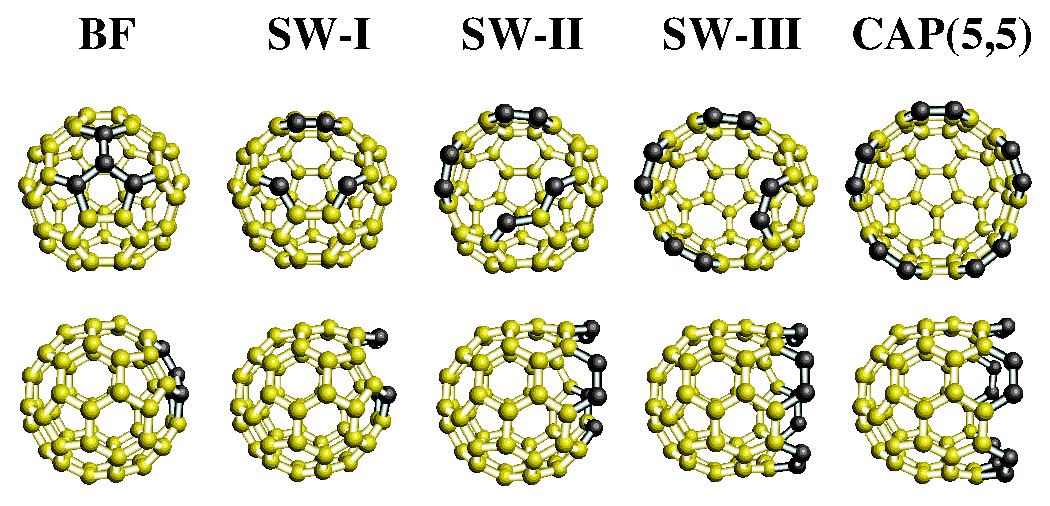
\includegraphics[width=0.5\textwidth]{figures/sample-fig1}
%	\label{fig:sample}
%	\caption{Sample Figure}
%\end{figure}
%
%\section{Answer to RQ2 : Computational simulation predicts causal relationship of exceed motor command in M1 from VL in Parkinson’s disease patient}
%
%\subsection{ The high synchronization (correlated neural activities) in VL but not average firing rate can drive M1’s motor command}
%
%
%Figure .2.1 The high synchronized neural activities during bursting can drive M1 in WT types but not KO, even though the average firing rate if WT and KO are not significantly difference
%
%
%\subsection{ The high synchronization level can be achieved by bursting. The demolishing of bursting in WT neurons result in the absent of synchronization in neuron population}
%
%Figure .2.2 Schematic diagram of how the bursting activity cause high synchronization in neuron population
%
%\subsection{ The Analysis of information transfer from VL to M1 : The information in VL can transfer to M1 when the neuron population in VL are synchronized }
%
%Figure .2.3 the neural information from VL is transferring to M1 only when the neural activities in VL are synchronized.
%
%Figure .2.4 the level of information transfer between VL and M1 is proportionally to the synchronization level in VL
%
%\subsection{ Artificially generated bursting in KO neurons result in high synchronization level of neuron population which can drive M1’s motor command
%}
%Figure .2.5 successfully generated bursting behavior in KO with similar bursting behavior generated by T-Type Calcium channel in WT
%
%Figure .2.6 The artificial bursting behavior in KO result in high level synchronization level of neural population and this high synchronized neural 
%population can drive M1
%
%\subsection{ Artificially activated VL neural population in theta and beta frequencies result in motor command from M1with the same frequency band with what observed in Parkinson’s disease patient.}
%


%%
%% 표 삽입 예시
%% Example. how to insert table
%%
\begin{table}[t]
\caption{Energy stability $E$ (eV) per molecule of all meta-stable
isomer states of C$_{60}$ opening process for forming the (5,5) cap.
In the SW-I and SW-II, both ferromagnetic (Ferro) and paramagnetic (Para)
spin configurations are obtained, whereas only non-magnetic configuration
is obtained in the BF, SW-III, and CAP(5,5).
$M$ is total magnetization $n_{\rm up}$-$n_{\rm down}$ in unit of $\mu_B$, where
$n_{\rm up(down)}$ is the number of up (down) spins.
}
\label{mag-tab1}
\begin{center}
\begin{tabular} {ccccccccccc}
\hline\hline
& & BF &\multicolumn{2}{c}{SW-I}&&\multicolumn{2}{c}{SW-II}&SW-III&CAP&\\
\cline{4-5} \cline{7-8}
&               &   &  Para & Ferro &&   Para &  Ferro &      &      &\\
\hline
& $E$ (eV)      & 0 & 7.796 & 7.832 && 10.418 & 10.408 & 11.5 & 13.2 &\\
& $M$ ($\mu_B$) & 0 &     0 &  1.94 &&      0 &   2.06 &    0 &    0 &\\
\hline\hline
\end{tabular}
\end{center}
\end{table}


%%
%% 그림 삽입 예시
%% Example. how to insert graph
%%
%% Note. 가급적 \includegraphics 명령을 사용하십시오.
%% Recommen : Use \includegraphics to insert graph.
%%

\chapter{Conclusion}

This work introduced the generalised model for neural network simulation. The model acts as a template for simulation study that does not limited to only this paper, but also any other neural network models. Using this generalised model, a model for study on the modulation of information transfer in feedforward network was made. 
In order to study how information transfer can be modulated in the feedforward networks, three levels of input synchronization were given to the target layer under three convergent connection rules (GG, UU, UE). In this work, we studied the modulation of information transfer by mean of the output firing rate that appears when input changes from static to oscillating input.

First, we show that feedforward network under various types of input and various types of convergent connections rules has distinct activity map for each condition.
We then show an increase in the output firing rate when the feedforward connection strength increases and when the synchronization level during the input increases. We demonstrate that the Uniform-Uniform convergent rule (UU) has the highest response gain from a static input to an oscillating input when compared to other convergent rules. Finally, we reveal that the UU rule has the highest induced spike gain and that it is highly dependent on the phase of the input oscillation. An explanation of why the UU rule is most sensitive to synchronized input based on the idea of temporal summation was also given.

In summary, we found that high level of synchronization in input results in high output response and the synchronized input can make a specific level of output with low cost of connection compared to the static input. In addition, neural network with Uniform-Uniform convergent connection rule is selective to change in input synchronization compared to the other two rules. These results suggest that both input synchronization level and the interlayer connection rules can contribute to the understanding of brain connections. 

\paragraph{} 


%What does it mean?
%Successfully regenerate experimental results with computational simulation
%The simulation shows functional connection between thalamus and motor cortex in the real animal
%What hypotheses were proved or disproved?
%We can make computational simulation which resemble the experimental data
%The T-Type calcium channel generate bursting behavior of single cell
%The neural population are highly synchronized during bursting behavior
%The high synchronization level in neural population can transfer information from one layer to another layer
%What did I learn?
%I can make computational model that can regenerate experimental data and I can use it to predict new properties of neural system
%Why does it make a differences?
%The simulation predicts functional connection between VL and M1 neuronal layers
%The simulation suggest that reverse testing of KO cells to resemble WT can also drive motor command in M1. The finding suggests that the bursting is the important factor for high synchronization level of neural population and it is the key for neural network to transfer data from VL to M1
%
%Add a new, higher level of analysis
%Indicate explicitly the significance of the work
%This work shows the potential of using computational simulation to regenerate experimental data in silico and employ it to manipulate properties of neuron network that are hard to do in the experiments and use it to predict new hypothesis


%%
%% 참고문헌 시작
%% References
%%

%\begin{thebibliography}{00}
%
%\bibitem{Iijima91} S. Iijima,
%         Nature (London) {\bf 354}, 56 (1991).
%         %Helical microtubules of graphitic carbon.
%
%\bibitem{Dresselhaus96} M. S. Dresselhaus, G. Dresselhaus, and P. C. Eklund.
%         {\em Science of Fullerenes and Carbon Nanotubes} (Academic, San Diego, 1996).
%
%\bibitem{Saito98} R. Saito, G. Dresselhaus, and M. S. Dresselhaus,
%         {\em Physical Properties of Carbon Nanotubes}
%         (Imperial College Press, London, 1998).
%
%\bibitem{Makarova01} T.L. Makarova, B. Sundqvist,
%         R. H\"ohne, P. Esquinazi, Y. Kopelevich, P. Scharff,
%         V.A. Davydov, L.S. Kashevarova, and A.V. Rakhmanina,
%         Nature (London) {\bf 413}, 716 (2001).
%
%\bibitem{Palacio01} F. Palacio, Nature (London) {\bf 413}, 690 (2001),
%         and references therein.
%
%\bibitem{SW} A.J. Stone and D.J. Wales,
%         Chem. Phys. Lett {\bf 128}, 501 (1986).
%
%\end{thebibliography}

\bibliographystyle{naturemag}
\bibliography{references}

%%
%% 한글요약문 시작 (Korean summary)
%%
%% Note. 영문논문일 경우에만 필요하니 한글논문의 경우에는 작성하지 마십시오.
%%
\begin{summary}

    지난 10여 년간 탄소 나노튜브는 자체의 독특한 전기적, 기계적 성질로
    인하여 다가오는 나노기술 분야의 이상적인 기초물질중의 하나로 떠오르고
    있다. 흑연을 감는 세세한 방법에 따라 전기적 특성이 금속성에서 1eV의
    띠간격을 가지는 반도체 특성까지 다양한 분포로 존재한다.
    본 학위논문에서는 탄소 나노튜브의 여러 물리적 성질에 대해 고찰하는데,
    기본적으로 제일원리 밀도함수 이론과 밀접결합근사 모형을 사용하여 전기적
    특성과 그 제어 방법, 자기적 특성, 그리고 수송특성 등을 다루고자 한다.

\end{summary}

%%
%% 감사의 글 시작
%% Acknowledgement
%%
% @command acknowledgement 감사의글
% @options [default: 클래스 옵션 korean|english ]
% - korean : 한글타이틀 | english : 영문타이틀

\acknowledgement[korean]

    이 논문을 완성하기까지 주위의 모든 분들로부터 수많은 도움을 받았습니다.

    끝으로 오늘의 제가 있을 수 있도록 사랑으로 키워 주신
    어머니와 또한 가족들에게 감사드립니다.
    저의 이 작은 결실이 그분들께 조금이나마 보답이 되기를 바랍니다.

%%
%% 이력서 시작
%% Curriculum Vitae
%%
% @command curriculumvitae 이력서
% @options [default: 클래스 옵션 korean|english ]
% - korean : 한글이력서 | english : 영문이력서
\curriculumvitae[korean]

    % @environment personaldata 개인정보
    % @command     name         이름
    %              dateofbirth  생년월일
    %              birthplace   출생지
    %              domicile     본적지
    %              address      주소지
    %              email        E-mail 주소
    % - 위 6개의 기본 필드 중에 이력서에 적고 싶은 정보를 입력
    % input data only you want
    \begin{personaldata}
        \name       {김 용 현}
        \dateofbirth{1972}{3}{25}
        \birthplace {대전 대덕구 평촌동 ...}
        \domicile   {대전 유성구 신성동 ...}
        \address    {대전 유성구 구성동 ...}
        \email      {yonghyunkim@test.kaist.ac.kr}
    \end{personaldata}

    % @environment education 학력
    % @options [default: (none)] - 수학기간을 입력
    \begin{education}
        \item[1988. 3.\ --\ 1990. 2.] 대전과학고등학교 (2년 수료)
        \item[1990. 3.\ --\ 1997. 2.] 한국과학기술원 물리학과 (B.S.)
        \item[1997. 3.\ --\ 1999. 2.] 한국과학기술원 물리학과 (M.S.)
    \end{education}

    % @environment career 경력
    % @options [default: (none)] - 해당기간을 입력
    \begin{career}
        \item[1997. 3.\ --\ 1999. 2.] 한국과학기술원 물리학과 일반조교
        \item[2001. 7.\ --\ 2002. 1.] 한국과학기술정보연구원 슈퍼컴퓨팅센터 위촉연구원
        \item[2002. 8.\ --\ 2002. 12.] 한국표준과학연구원 연구생
    \end{career}

    % @environment activity 학회활동
    % @options [default: (none)] - 활동내용을 입력
    \begin{activity}
        \item J. Choi, \textbf{Yong-Hyun Kim}, K.J. Chang, and D. Tomanek,
             \textit{Occurrence of itinerant ferromagnetism in C/BN superlattice
             nanotubes}, 5th Asian Workshop on First-Principles Electronic
             Structure Calculations, Seoul (Korea), October., 2002.
    \end{activity}

    % @environment publication 연구업적
    % @options [default: (none)] - 출판내용을 입력
    \begin{publication}
        \item \textbf{Yong-Hyun Kim}, J. Choi, K.J. Chang, and D. Tomanek,
             \textit{Magnetic instability in partly opened C$_{60}$ isomers},
             in preparation.
    \end{publication}

%% 본문 끝
\end{document}
